\section{Off-energy Orbits}\label{sec:3.1}

In the preceding sections I have been discussing the trajectories in a storage ring of electrons with the nominal energy $E_0$ -- which is the design energy for a given setting of the magnet currents. Stored electrons do not, however, all have this ideal energy. In general, the energy $E$ of a stored electron will deviate from the nominal energy, and, as described in Section~\ref{sec:1.2}, will oscillate about it. These energy oscillations - often called “synchrotron oscillations” - are the subject of the part.\\
We must, first, understand the motion of electrons whose energy differs by a small amount $\epsilon$ from the nominal energy. Keeping the assumptions of Section~\ref{sec:2.3} that the design orbit lies in a horizontal plane, energy deviations will, to first order in small quantities, affect only the radial motion. The vertical displacement will still be described by the betatron oscillations analyzed in Chapter 2, and will not be considered further here. From Section~\ref{sec:2.6} onward it was convenient to-let the symbol $x$ stand generally for either $x_\beta$ or $y_\beta$ the lateral displacements associated with the betatron oscillations. I now return to the notation in which $x$ represents the \emph{total horizontal} displacement of a trajectory from the design orbit.\\
It was shown in Section~\ref{sec:2.5} that in an ideal guide field the radial motion for
an electron with the energy deviation $\epsilon$ can be written as the sum of two parts
\begin{align}
	x = x_\beta+x_\epsilon,
\end{align}
where $x_\beta$ is the betatron displacement and $x_\epsilon$ is a displacement which depends
only on the energy of the electron. If we wish to include also the results of Section~\ref{sec:2.11}, we should include in addition, the distortion of the closed orbit due to magnet imperfections and write
\begin{align}
	x = x_\beta+x_\epsilon+x_c.
\end{align}
Since the various contributions add linearly -- under our assumptions of a linear guide field, of
 small energy deviations, and of small displacements -- we have been able to consider separately
 the several contributions to $x$. We now ignore the other contributions to $x$ and focus on $x_\epsilon$.
According to Eq.~\eqref{eq:2.28} the energy displacement $x_\epsilon$ can be written as a function of the variation of energy $\delta = \epsilon/E_0$ as follows
\begin{align} \label{eq:3.3}
	x_\epsilon = \eta(s) \delta.
\end{align}
where $\eta(s)$ is a function of the azimuthal coordinate $s$ which is single valued at
each physical azimuth. A off-energy electron with no betatron oscillations runs around a new closed orbit whose displacement from the ideal orbit is everywhere proportional to $\delta$, with a proportionality factor which depends on the azimuth according to a given function $\eta(s)$, characteristic of the total guide field configuration. I shall call $\eta(s)$ the dispersion function -- it is just the closed orbit displacement per unit energy deviation.\\
Let’s look now at the nature of $\eta(s)$. It was defined -- see Eq.~\eqref{eq:2.29} -- as that
solution of the differential equation\footnote{$\eta' = d\eta/ds.$}
\begin{align}\label{eq:3.4}
	\eta'' = -K_x\eta + G(s),
\end{align}
which is $L$-periodic in $s$ and is, therefore, single valued for all physical azimuths . The functions $G(s)$ and $K_x(s)$ were defined in Eqs. \eqref{eq:2.3} and \eqref{eq:2.21}.\\
Let’s consider the qualitative behavior implied by this equation for the $\eta(s)$ of a separated function guide field (which was defined in Section~\ref{sec:2.2}. We may take
as an example the guide field of the SLAC proposal which was used for illustration in Sections \ref{sec:2.6} and \ref{sec:2.10}. In Fig. \ref{fig:fig29}(a), (b) I show $K_x$ and $G$ for this guide field and in (c), the dispersion function $\eta(s)$.
\begin{figure}[!htb]
	\centering
	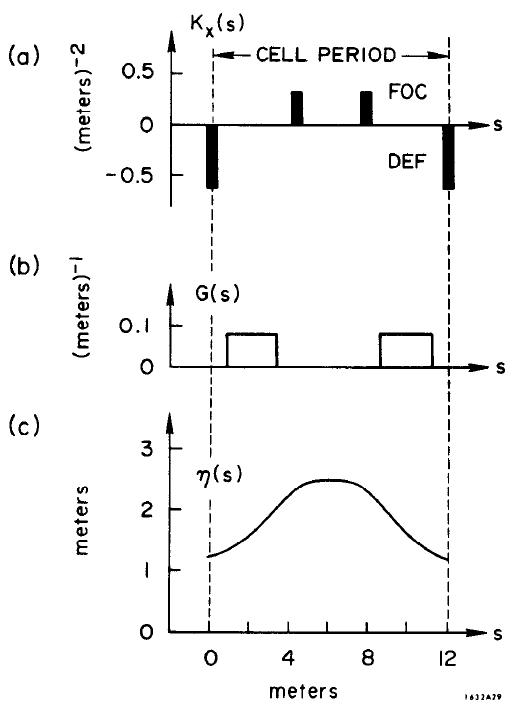
\includegraphics[width=0.8\linewidth]{./Figuras/fig29.jpeg}
	\caption{Guide-field functions and the off-momentum function for the SLAC guide field.}
	\label{fig:fig29}
\end{figure}
In a field free section both $G$ and $K_x$ are zero so $\eta(s)$ has a segment of constant
slope. In a pure quadrupole $G$ is zero and $K_x$ is just the quadrupole strength. In
a focusing quadrupole $K_x$ is positive and $\eta(s)$ follows a segment of a sinusoidal
oscillation about zero with the form
\begin{align*}
	\eta = a \cos(\sqrt{K_x}s + \vartheta).
\end{align*}
In a defocusing quadrupole $K_x$ is negative and $\eta(s)$ follows a segment of a positive
exponential like
\begin{align*}
	\eta = a \cosh(\sqrt{-K_x}s+\vartheta).
\end{align*}
The curve of $\eta(s)$ is ``attracted'' toward the $s$-axis in a focusing quad and repelled
from the axis in a defocusing quad.
Although $K_1$ is zero in a flat bending magnet, $K_x$ is not. In fact, $K_x = G^2$ and
the equation for $\eta$ is
\begin{align}
	\eta'' = -G^2\eta + G = -G^2\left( \eta - \dfrac{1}{G} \right).
\end{align}
The curve of $\eta$ is a segment of a sinusoid which is ``attracted'' toward the level
$\eta_0 = 1/G$ with a ``restoring force'' proportional to $G^2$ (The level $\eta_0$ is just equal
to the radius of curvature $\rho$ of the design orbit).\\
From the above discussion you can understand the qualitative features of the variations
 of $\eta(s)$ that appear in Fig.~\ref{fig:fig29}. For all ``normal'' storage rings it turns
out that the dispersion function is everywhere positive.\\
A storage ring user is not generally faced with the need to make a detailed calculation of $\eta(s)$. Its graph should be provided by the ring designers. I will therefore, only indicate briefly how it may be calculated. For a separated function guide field the preceding discussion can be expanded to give a method for calculating $\eta(s)$. Suppose you begin at $s = 0$ with some assumed values of $\eta(0)$ and $\eta'(0)$ and evaluate $\eta(s)$ as a succession of segments of the kind described above until you make your way around one complete revolution -- until you get to $s = L$. You will get the true $\eta(s)$ if you then choose $\eta(0)$ and $\eta'(0)$ so that $\eta(L)$ and $\eta'(L)$ are respectively, equal to $\eta(0)$ and $\eta'(0)$. The computation can be carried out most straightforwardly by using a matrix technique (See Ref. \cite{11}).\\
The dispersion function can also be obtained (for any kind of guide field) by making use of the results we obtained in Section~\ref{sec:2.11} for disturbed closed orbits. We may imagine that an off-energy orbit is just a ``disturbed'' closed orbit since an energy deviation gives rise to a change in curvature just as does a field error. That is to say, that a field error $\delta G$ in a segment $\Delta s$ of the orbit produces a change of curvature in the path of an electron of energy $E_0$ which is the same as the change of curvature that results when an electron with an energy deviation $\delta$ goes through the nominal field provided that $\delta G/G = \delta$. Since $\eta(s)$ is the ratio of the closed orbit displacement to $\delta$, we may compute $\eta(s)$ by replacing $\delta G$ in Eq.~\eqref{eq:2.92} of Section~\ref{sec:2.11} by $G$. This argument can also be justified by noticing that Eq.~\eqref{eq:3.4} for $\eta$ has the same form as Eq.~\eqref{eq:2.85} for $x_c$ in Section~\ref{sec:2.11}; the latter going into the former
 if we make the substitutions $x_c \to \eta$ and $\delta G \to G$. Making the same substitutions
 in Eq.~\eqref{eq:2.94} we get
\begin{align}
	\boxed{ \eta(s) = \dfrac{\sqrt{\beta(s)}}{2\sin\pi\nu}\oint G(\bar{s})\sqrt{\beta(\bar{s})}\cos\left\lbrace |\varphi(s) - \varphi(\bar{s})| - \pi\nu \right\rbrace d\bar{s}}.
\end{align}
So if $\beta(s)$ is already known we can get $\eta(s)$ by an integration. Notice that $\eta(s)$ too will have a resonance behavior when $\nu$ approaches an integer.\\
If the design orbit does not lie in a plane - as, for example, in the recent DESY or Orsay designs - then the discussion of this Section must be repeated for the vertical displacements.
 There will in such cases be two curvature functions $G_x$ and $G_y$ as well as the two focussing functions $K_x$ and $K_y$. The vertical displacements will also have an off-energy contribution which will be proportional to an dispersion function $\eta_y(s)$. And this vertical
 dispersion function can be evaluated in terms of the vertical focusing and curvature functions.
 There will be generally one important qualitative difference from the horizontal case in that $\eta_y$, will have both positive and negative values and its average around the ring will be zero.
